\chapter{Algorithm development}
In the analysis we have chosen to use audio to measure the distance. As the main principle is to use the speed of sound to calculate the distance, we will need to play some audio and record it when it returns. The task is then to calculate the time elapsed between the moment we play it and the moment we record it. The algorithm should be able to recognize the signal as it returns. 

The ultimate goal is to have a function that - when given the two data sets - would provide the distance to the specific object.

When getting to know an algorithm it is useful to use it with well-known, manageable data, such as:
\\
Green: [0,1,2,1,0,0,0]\\
Blue: [0,0,0,1,2,1,0]\\
The green data set simulates our output audio and the blue data set simulates the recorded audio. When plotting the two signals, we get figure \ref{fig:xcrossSample}. Because the data sets are so small it is very easy to see that the two signals are identical when shifting the blue data set two elements to the left. Our algorithm, cross-correlation, should be able to calculate that. We could either make our own or use an existing. We quickly got to know cross-correlation which was perfect for our needs

\section{Cross-correlation}
The cross-correlation algorithm is used for searching a data set for specific features, patterns or identical signals.

Cross-correlation starts with the rightmost element of one of the data sets and multiplies this value with the leftmost  element of the second data set. This is then stored and the next step is done. The next step is to multiply the rightmost  element with the second leftmost element of the second data set and then added to the result of the multiplication of the  leftmost element in the first data set and the second rightmost element of the second set. This means that the element in the result-data set is the result of one multiplication, then two multiplications added, three multiplications added up till a result consisting of the sum of N multiplications where N is the size of the data set that is outputted. Depending on the size of the recorded audio there might be several results consisting of the sum of N multiplications. Eventually there will be N-1 multiplications and then down until there is only one multiplication again - this time on the other side of the data set.

Because of this symmetry the result-data set will have a length of N-1 in the range of -N to N.

The equation in \ref{eq:xcross} is the mathematical expression fo cross-correlation of discrete functions.
\begin{equation}
\label{eq:xcross}
\centering
(f\star g)(t)=\sum\limits_{m=-\infty}^{m=\infty}f(t)*g(t+m)
\end{equation}

Instead of letting m be in the range of $-\infty$ to $\infty$, we will let our sample size control the range, as in equation \ref{eq:xcrossN}

\begin{equation}
\label{eq:xcross2}
\centering
(f\star g)(t)=\sum\limits_{m=-7}^{m=7}f(t)*g(t+m)
\end{equation}

\begin{equation}
\label{eq:xcrossN}
\centering
(f\star g)(t)=\sum\limits_{m=-N}^{m=N}f(t)*g(t+m)
\end{equation}

Normally, cross-correlation will calculate a negative counterpart in the case that the signal is shifted to the left instead of to the right (the signal is shifted right in \ref{eq:xcrossSample}). Since we in our setup record the audio and then compare the recording with the output we can rule out any left-shifting of the signal. We can do so simply because audio can not be recorded before it has been played. This is an important step in optimization because we have just halved  the amount of operations needed.

Therefore we will have t in the range of $t=0$ to $t=7$. 

We can then, following equation \ref{eq:xcross2}, calculate the cross-correlation:

\begin{center}
$(f\star g)(0)=f(0)*g(0+(-7)+f(0)*g(0+(-6))+...+f(0)*g(0+6)+f(0)*g(0+7)$\\
$(f\star g)(1)=f(1)*g(1+(-7)+f(1)*g(1+(-6))+...+f(1)*g(1+6)+f(1)*g(1+7)$\\
$(f\star g)(2)=f(2)*g(2+(-7)+f(2)*g(2+(-6))+...+f(2)*g(2+6)+f(2)*g(2+7)$\\
$...$\\
$(f\star g)(6)=f(6)*g(6+(-7)+f(6)*g(6+(-6))+...+f(6)*g(2+6)+f(6)*g(6+7)$\\
$(f\star g)(7)=f(7)*g(7+(-7)+f(7)*g(7+(-6))+...+f(7)*g(3+6)+f(7)*g(7+7)$\\
\ \\
$(f\star g)(0:7)=[1\ 4\ 6\ 4\ 1\ 0\ 0\ 0]$\\
\end{center}

Because of the nature of the math in the cross-correlation we will have the highest value in the element with the value identical to the times the recorded signal has to be shifted to the left in order to be identical to the output signal. This can be used to calculate the distance. This will be further explained later in this chapter.

As we see the highest value is 6 in element 2 in the results data set. This fits with our initial thoughts.

The next step is to determine an implementation of the algorithm in MatLab. Once again we can choose to use an existing implementation or make our own. We did both.

The existing implementation is a function called xcorr. Xcorr, as used by us, takes two parameters: the recorded audio and the output. It returns a data set and a set with the t values from equation \ref{eq:xcross}.

\section{Signals}
To determine which signal type which was most favourable to use we made a script in matlab which generated 3 signal types, here one signal without a delay and one with a delay. This way we can analyse which signals would return the sharpest spike when cross correlated.
\subsection{Chirp}
A chirp is a signal which starts at a particular frequency and then changes the frequency fluently until it ends at another frequency.\\
Below is shown the code generating a chirp from 8kHz to 10kHz, then making a delayed version of this signal and lastly cross-correlating these signals.\\
\begin{lstlisting}[language=Matlab,frame=lrtb,label=Matlab Code for Chirp Cross-correlation]
Fs=48000;                                       % Sample frequency
t = [0:1/Fs:1];                                 % Timeinterval and length
Frq1=8000;                                      % Start frequency for chirp
Frq2=10000;                                     % End frequency for chirp
delay = 2000;                                   % Signal Delay
Chirp_signal=chirp(t,Frq1,1,Frq2);              % Chirp signal generation
Chirp_delayed=[zeros(1,delay) Chirp_signal];    % Chip delay generation
Chirp_xcorr=xcorr(Chirp_signal,Chirp_delayed);  % Cross-correlation
\end{lstlisting}
Below is the plot of the cross-correlation. It shows clearly where the to signal overlap.\\
\begin{figure}[H]
\begin{minipage}[b]{0.49\linewidth}
\centering
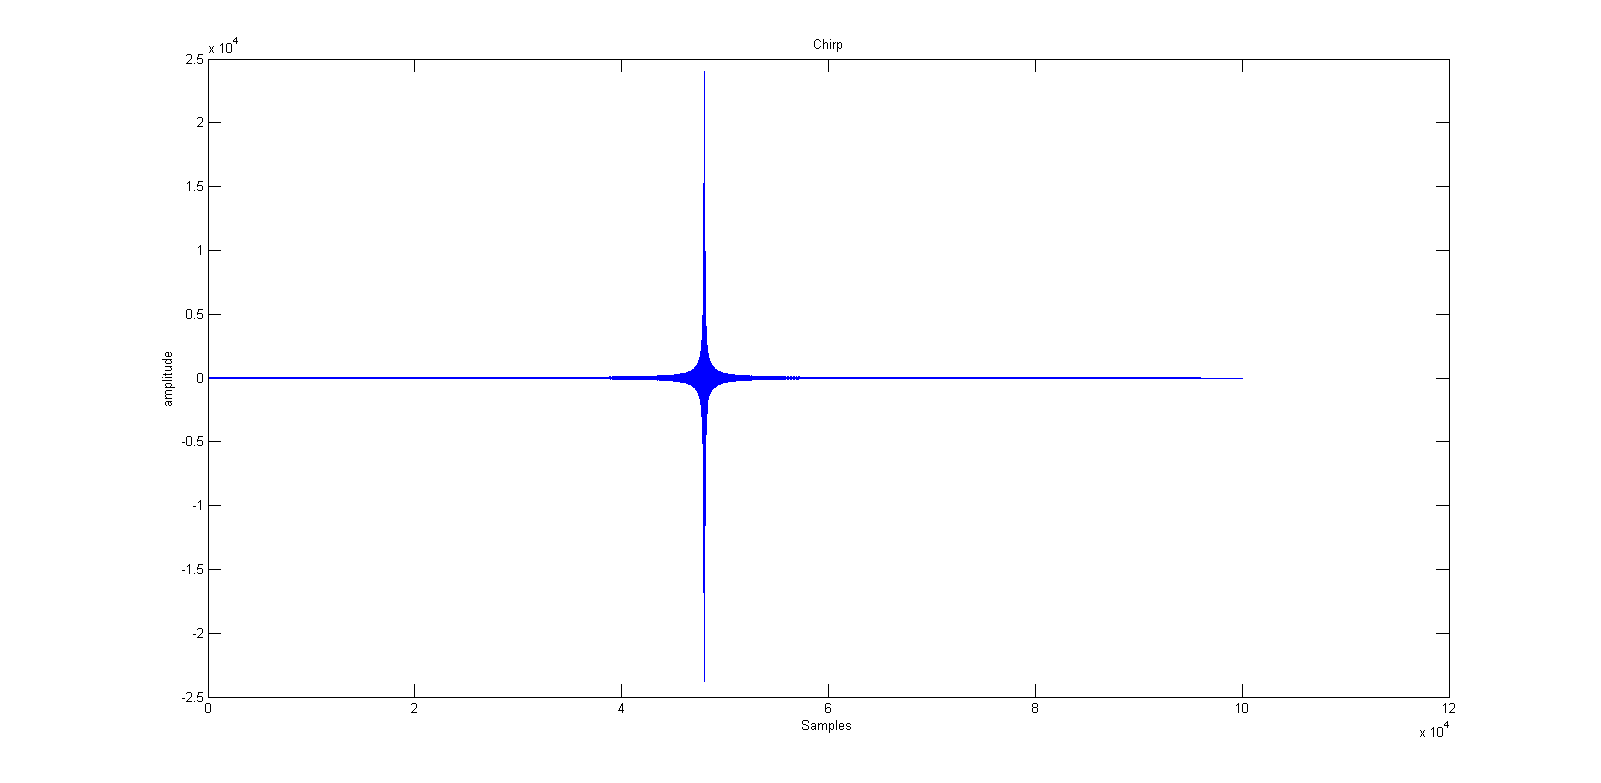
\includegraphics[width=1\textwidth]{billeder/chirp_xcorr_fig}
\caption{Chirp Cross-correlation}
\label{fig:figure1}
\end{minipage}
\hspace{0.5cm}
\begin{minipage}[b]{0.49\linewidth}
\centering
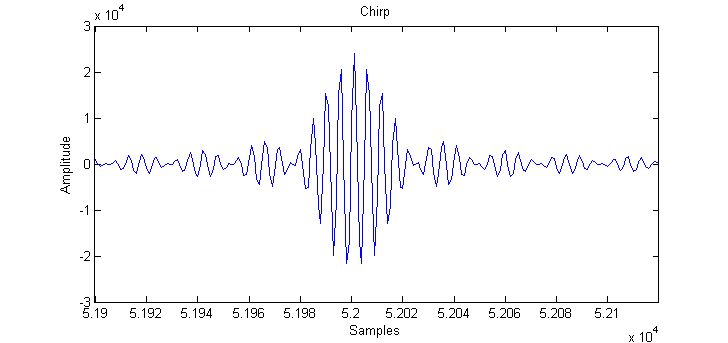
\includegraphics[width=1\textwidth]{billeder/chirp_xcorr_fig_zoom}
\caption{zoomed}
\label{fig:figure2}
\end{minipage}
\end{figure}
The Chirp seems like a solid signal to transmit. Since there exist a very specific area where it is clear the signals perfectly overlaps. The overlap shown above is centered around sample no. 52000 and spans around 10 samples.\\
This can easily be used to determine a somewhat precise distance. The distance of 10 samples @48kHz at the speed of sound is ~7cm.\\
Although matlab finds a precise sample for the max value we will have in mind that values close to the max is within the range of $\pm 3.5cm$.\\
\subsection{Sinusoid}
The initial thoughts about a sinusoid were mixed. Since a sinusoid overlaps more and more in periods we expect a triangle like cross-correlation. The sinus signals is treated the same way as the chirps in matlab and below is a plot of the cross-correlation.
\begin{figure}[H]
\begin{minipage}[b]{0.49\linewidth}
\centering
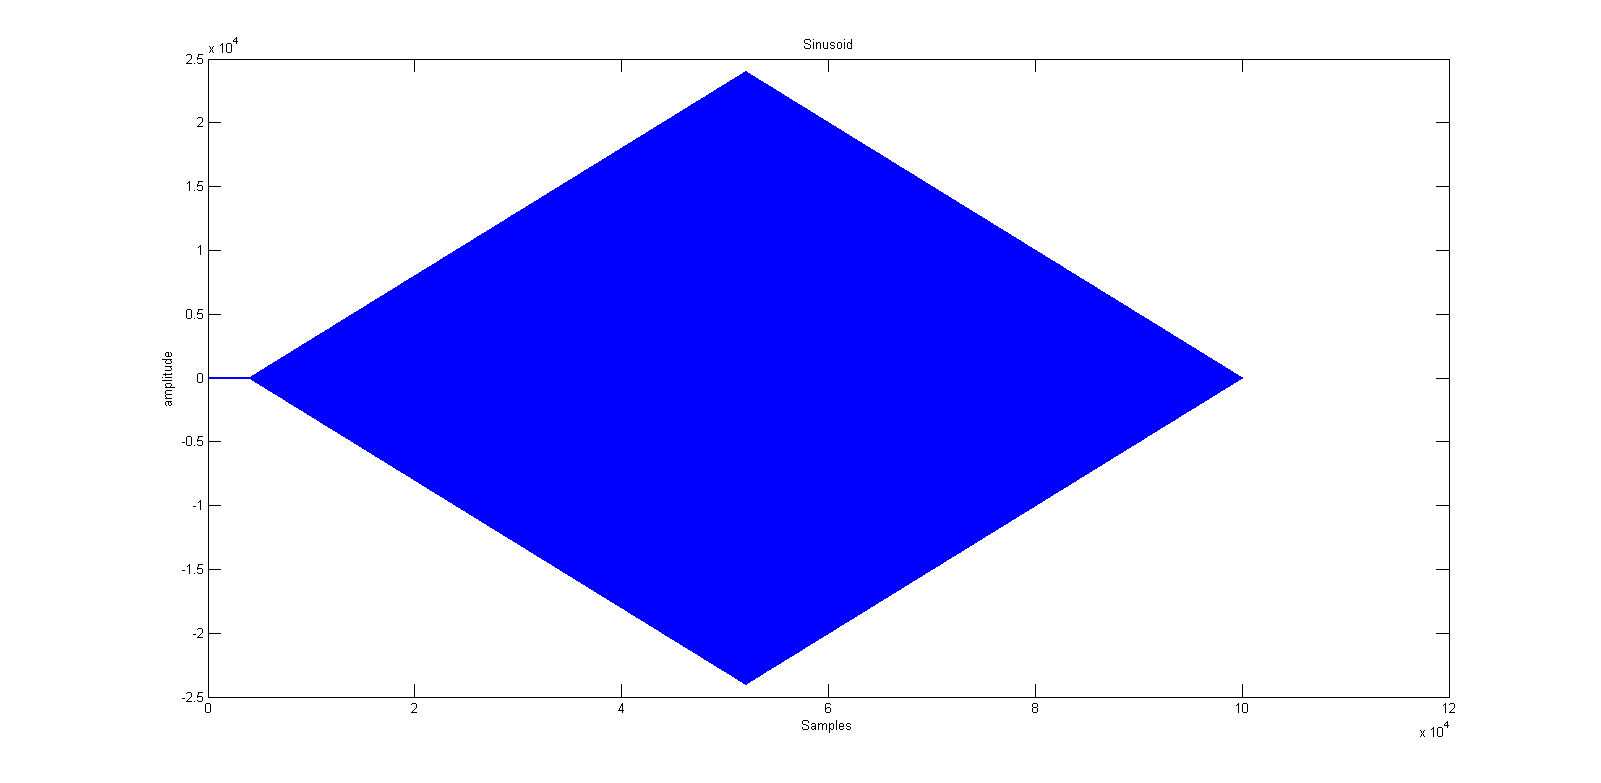
\includegraphics[width=1\textwidth]{billeder/sinus_xcorr_fig}
\caption{Sinusoid Cross-correlation}
\label{fig:figure1}
\end{minipage}
\hspace{0.5cm}
\begin{minipage}[b]{0.49\linewidth}
\centering
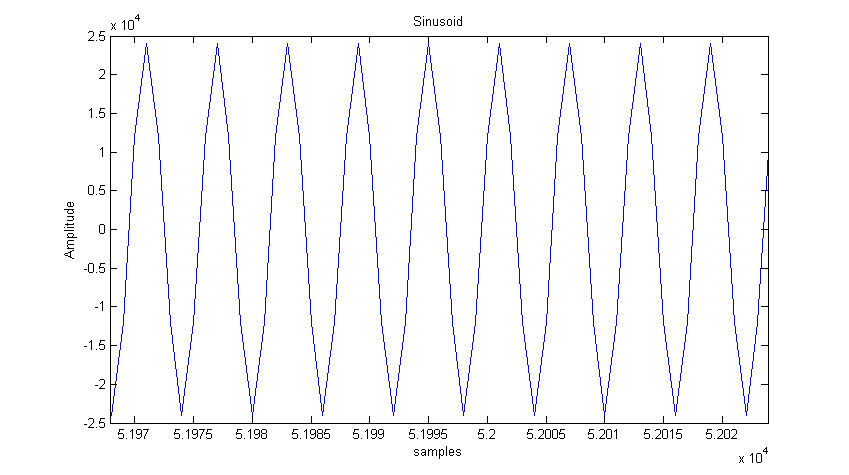
\includegraphics[width=1\textwidth]{billeder/sinus_xcorr_fig_zoom}
\caption{zoomed}
\label{fig:figure2}
\end{minipage}
\end{figure}
The zoomed plot is zoomed to the same window as the chirp signal. It is clear that the sinusoids peak isn't nearly as distinct as the chirp, hereby making the sinusoid signal less favourable. This also fits with our expectation since the sinusoid is very "simple" in shape compared to the chirp which is more unique.\\
\subsection{White noise}
Lastly we tried white noise. We expect this to be very distinct because the signal is very complex and consists of a lot of different frequencies. Therefore the signal will only overlay perfectly in one particular point. A noise signal was generated in matlab using the wgn() function. Below is a plot of the cross correlaltion.\\
\begin{figure}[H]
\begin{minipage}[b]{0.49\linewidth}
\centering
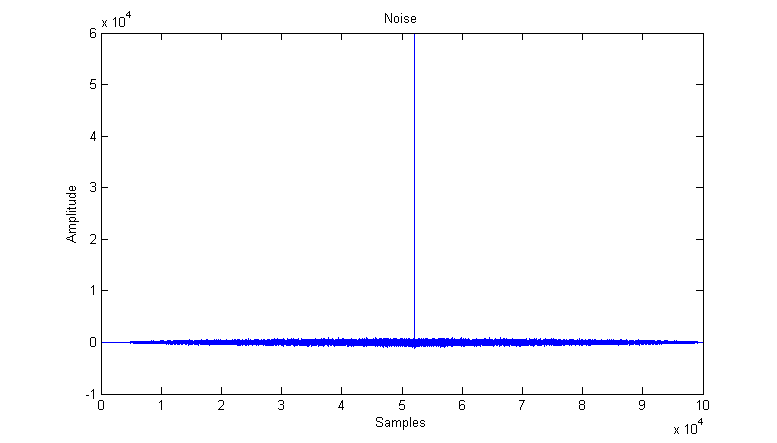
\includegraphics[width=1\textwidth]{billeder/noise_xcorr_fig}
\caption{Noise Cross-correlation}
\label{fig:figure1}
\end{minipage}
\hspace{0.5cm}
\begin{minipage}[b]{0.49\linewidth}
\centering
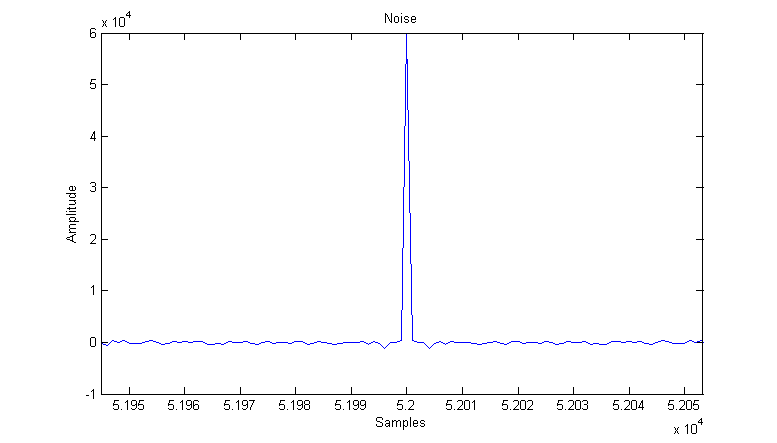
\includegraphics[width=1\textwidth]{billeder/noise_xcorr_fig_zoom}
\caption{zoomed}
\label{fig:figure2}
\end{minipage}
\end{figure}
As expected the noise was subject to a very sharp and distinct peak where the signals perfectly overlayed. The noise signals clearly seems like the best signal to transmit. The largest issue with the noise signal is that it is a very broad spectre. Since it is white noise it consists equally much of all signals.\\
\subsection{Robustness of signals}
%Her ligges der lidt støj ind over signalerne for at se hvor modstandsdygtige de er for støj.
As a last analysis of the signals we want to check the robustness of the signals. We want to do this by overlaying the generated signals with some noise. This is simply done in matlab by adding a noise signal to the original signal.\\
Before cross-correlating the signals an fft and a signal plot is made to ensure that the signals indeed have been overlayed with noise. Below is are these plots for the chirp.
\begin{figure}[H]
\begin{minipage}[b]{0.49\linewidth}
\centering
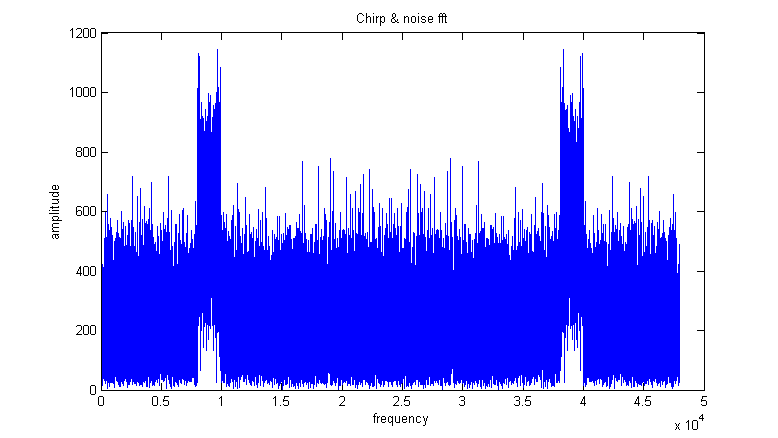
\includegraphics[width=1\textwidth]{billeder/chirp_noise_fft}
\caption{Chirp \& noise fft}
\label{fig:figure1}
\end{minipage}
\hspace{0.5cm}
\begin{minipage}[b]{0.49\linewidth}
\centering
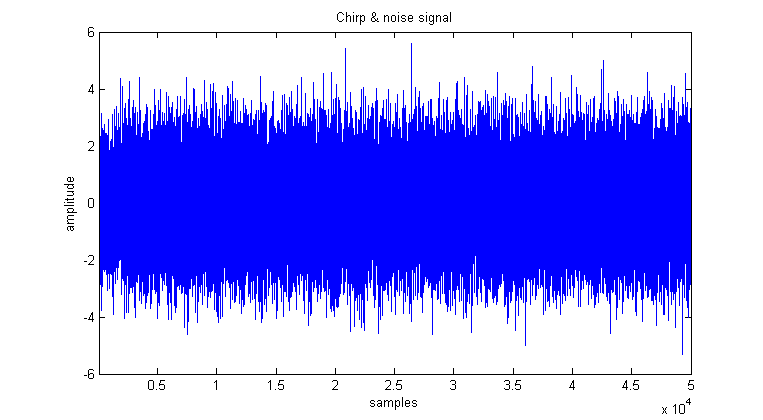
\includegraphics[width=1\textwidth]{billeder/chirp_noise_signal}
\caption{Chirp \& noise plot}
\label{fig:figure2}
\end{minipage}
\end{figure}
The fft plot shows that there is a lot of noise distributed over all frequencies but the original chirp is still present. The signal plot shows how much the chirp is disguised in the noise.\\
Below is a plot of the cross-correlation.
\begin{figure}[H]
\begin{minipage}[b]{0.49\linewidth}
\centering
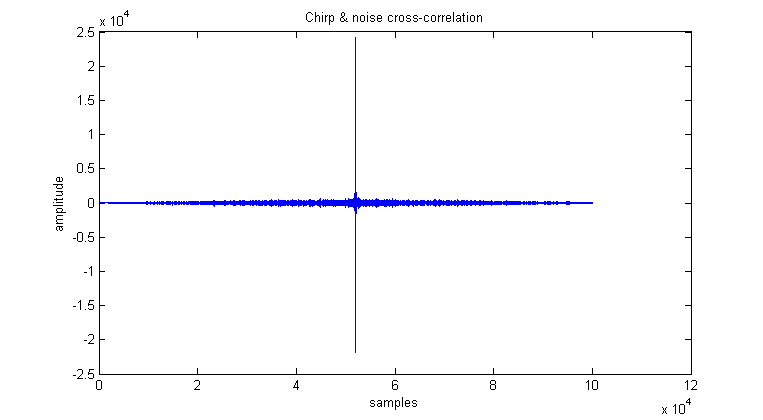
\includegraphics[width=1\textwidth]{billeder/chirp_noise_xcorr}
\caption{Chirp \& noise Cross-correlation}
\label{fig:figure1}
\end{minipage}
\hspace{0.5cm}
\begin{minipage}[b]{0.49\linewidth}
\centering
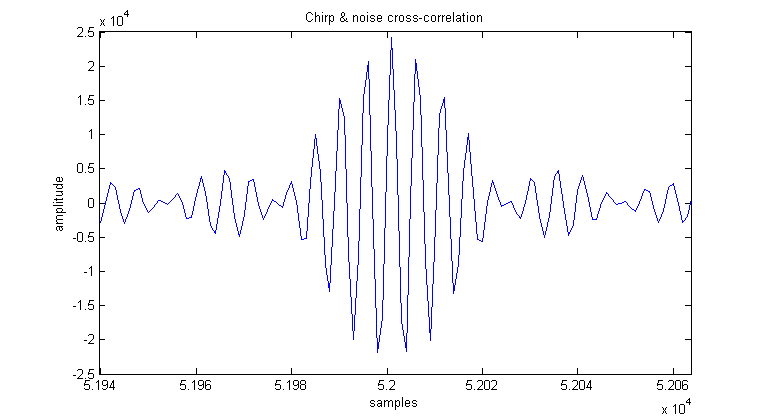
\includegraphics[width=1\textwidth]{billeder/chirp_noise_xcorr_zoom}
\caption{zoomed}
\label{fig:figure2}
\end{minipage}
\end{figure}
It is almost impossible to distinguish the noisy cross-correlation from the clean cross-correlation.\\